\subsection{Results}

Other methods for calculating local PCQA exist [REF-Leihui], but they tend to be very time-consuming. In contrast, our approach leverages a neural network to predict the surface density and quality directly, resulting in instantaneous predictions. In this method, the time-consuming part is the feature extraction step. This process is performed for the entire point cloud at once (without explicit loops), and its duration depends on the number of points in the point cloud. To measure this feature extraction time, point clouds of varying sizes were created using the Ball shape (Figure~\ref{fig:part_shapes_grid}). The results, shown in Figure~\ref{fig:time}, illustrate how the extraction time scales with point cloud size.

\begin{figure}[htbp]
\centering
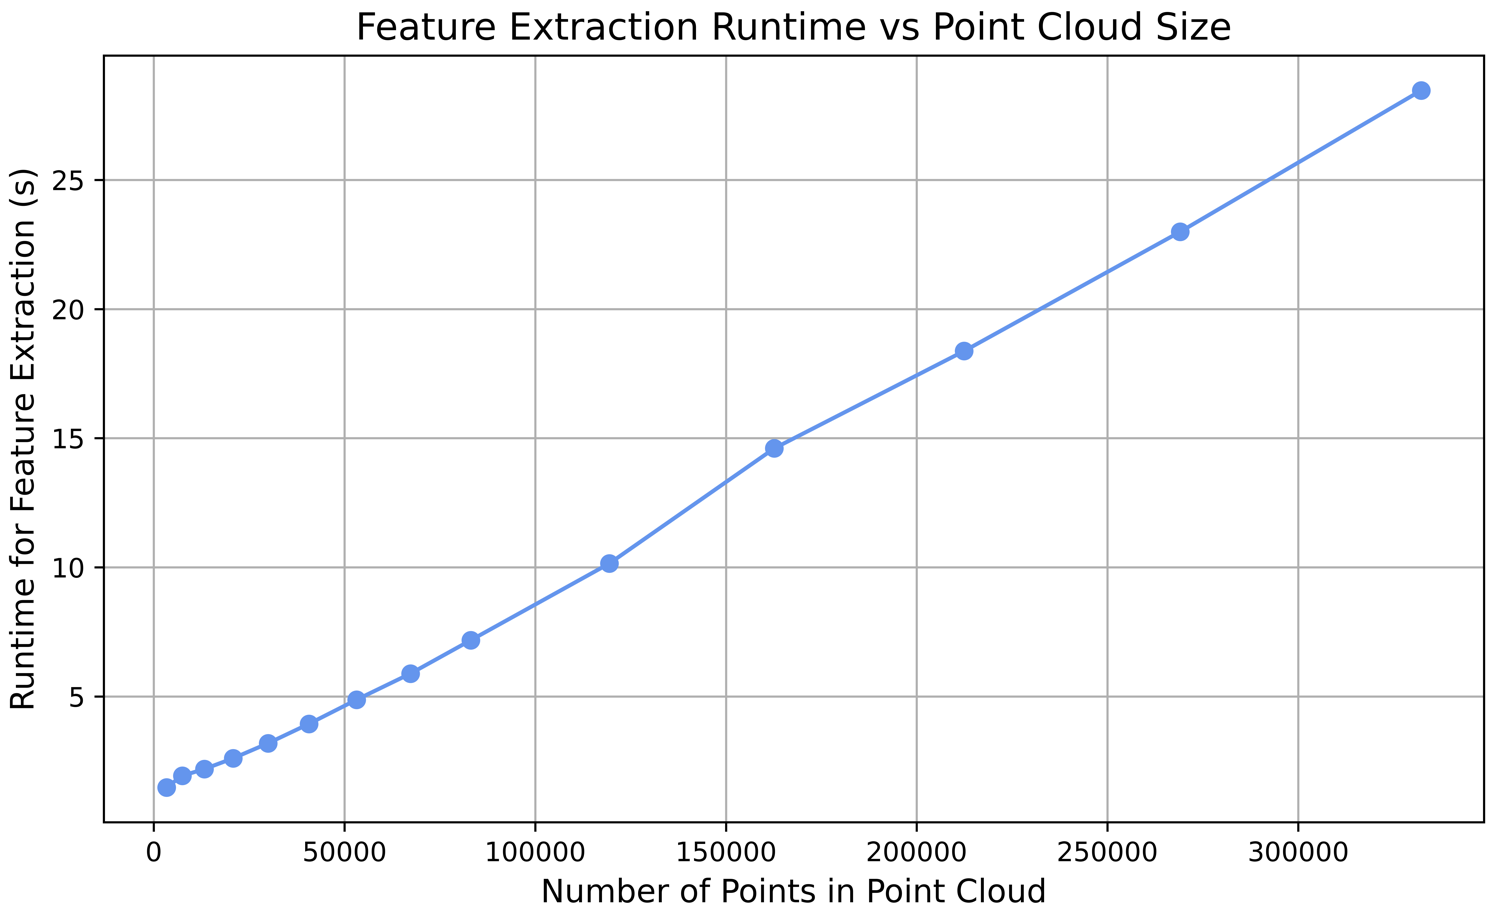
\includegraphics[width=0.5\textwidth]{figures/time_lowQ.png}
\caption{Feature extraction time consumption for different point cloud sizes.}
\label{fig:time}
\end{figure}

To evaluate the models trained on the two different datasets, the chainwheel shape was used to generate point clouds at various mesh sizes. For the model trained on dataset 1, predictions were very accurate for mesh sizes of 0.5 mm and again for sizes between 1 mm and 2 mm. However, mesh sizes between 0.6 mm and 1 mm showed larger prediction errors, with lower mean values and higher standard deviations, as seen in Figure~\ref{fig:pred_vs_label_first}.

\begin{figure}[H]
\centering
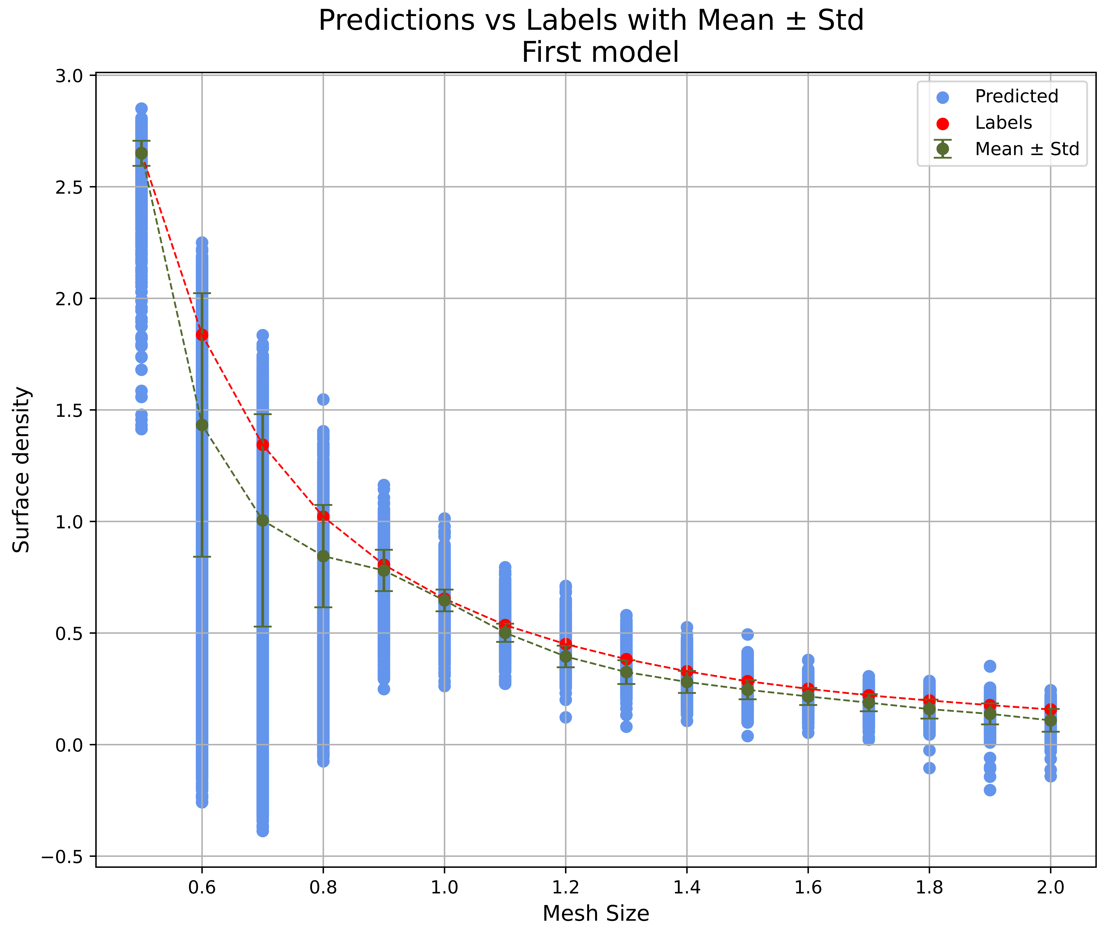
\includegraphics[width=0.5\textwidth]{figures/predict_vs_label_first_lowQ.png}
\caption{Predicted surface densities vs. ground truth labels. Model trained on 0.5, 1.0, and 2.0 mm mesh sizes.}
\label{fig:pred_vs_label_first}
\end{figure}

In contrast, the model trained on dataset 2 was much more robust, showing accurate predictions for all mesh sizes from 0.5 mm to 2 mm, with consistently low standard deviations (Figure~\ref{fig:pred_vs_label_better}). The variation in predictions also mirrored the expected variation in surface density across different mesh sizes, as seen in Figure~\ref{fig:sd_mesh}. Here, the variation in surface density is largest for the smallest mesh sizes and decreases as the mesh size increases.

\begin{figure}[H]
\centering
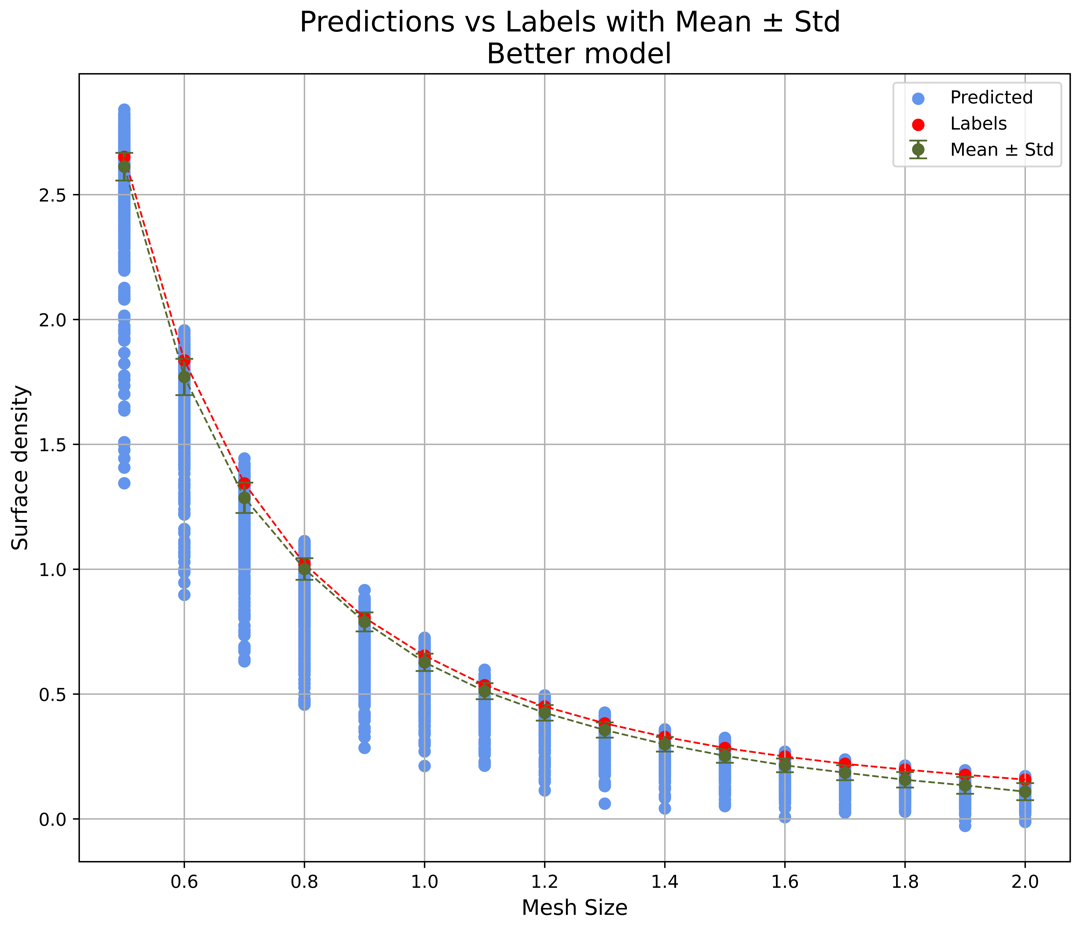
\includegraphics[width=0.5\textwidth]{figures/predict_vs_label_better_lowQ.png}
\caption{Predicted surface densities vs. ground truth labels. Model trained on 0.5 mm to 2.0 mm mesh sizes at 0.1 mm intervals.}
\label{fig:pred_vs_label_better}
\end{figure}

The model also successfully identifies areas of missing data, simulating the effect of an incomplete scan. To evaluate this, holes of varying sizes were introduced into the chainwheel point clouds, and the predicted surface density was analyzed. As seen in Figure~\ref{fig:holes_predict}, the model accurately marked these holes as regions of very low density—even detecting holes as small as five points. Notably, it also distinguished between actual part features and missing data; for example, the central hole in the chainwheel (which is a real feature) remained marked as a high-density region.

\begin{figure*}[t]
\centering
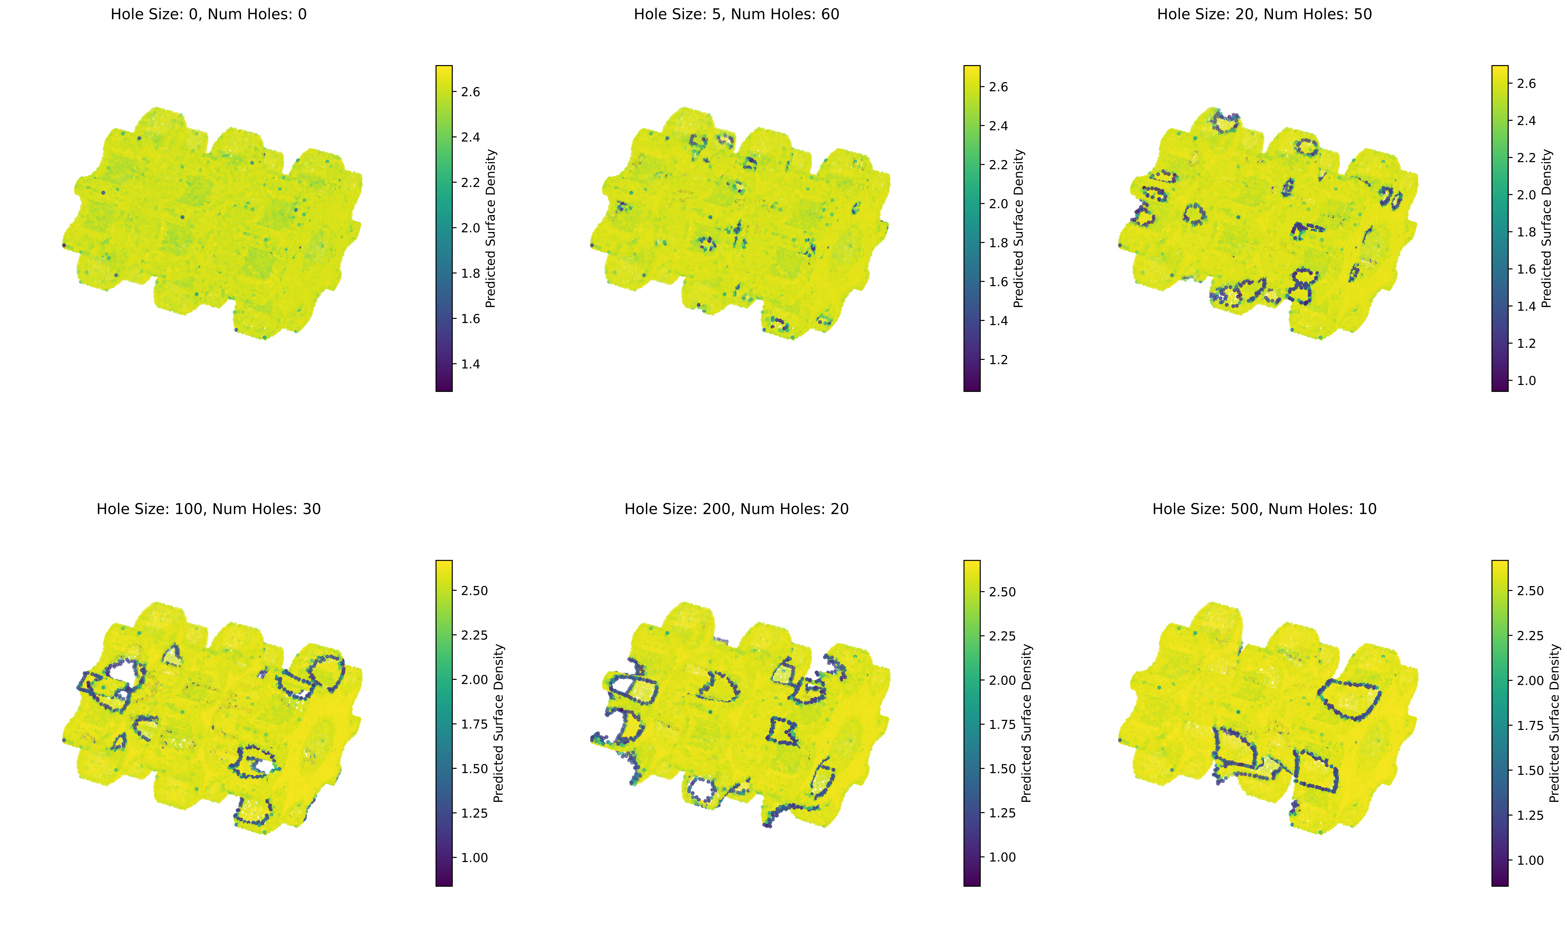
\includegraphics[width=\textwidth]{figures/result3_lowQ.png}
\caption{Surface density predictions for the same point cloud with varying hole sizes.}
\label{fig:holes_predict}
\end{figure*}

Finally, the model demonstrates impressive consistency in predicting varying surface densities within the same part. This is illustrated in Figure~\ref{fig:diff_mesh_predict}, where the chainwheel was segmented and meshed at different mesh sizes, but the entire point cloud was fed into the model as a single entity. The model accurately predicted the surface density variations corresponding to each mesh size segment.

\begin{figure}[H]
\centering
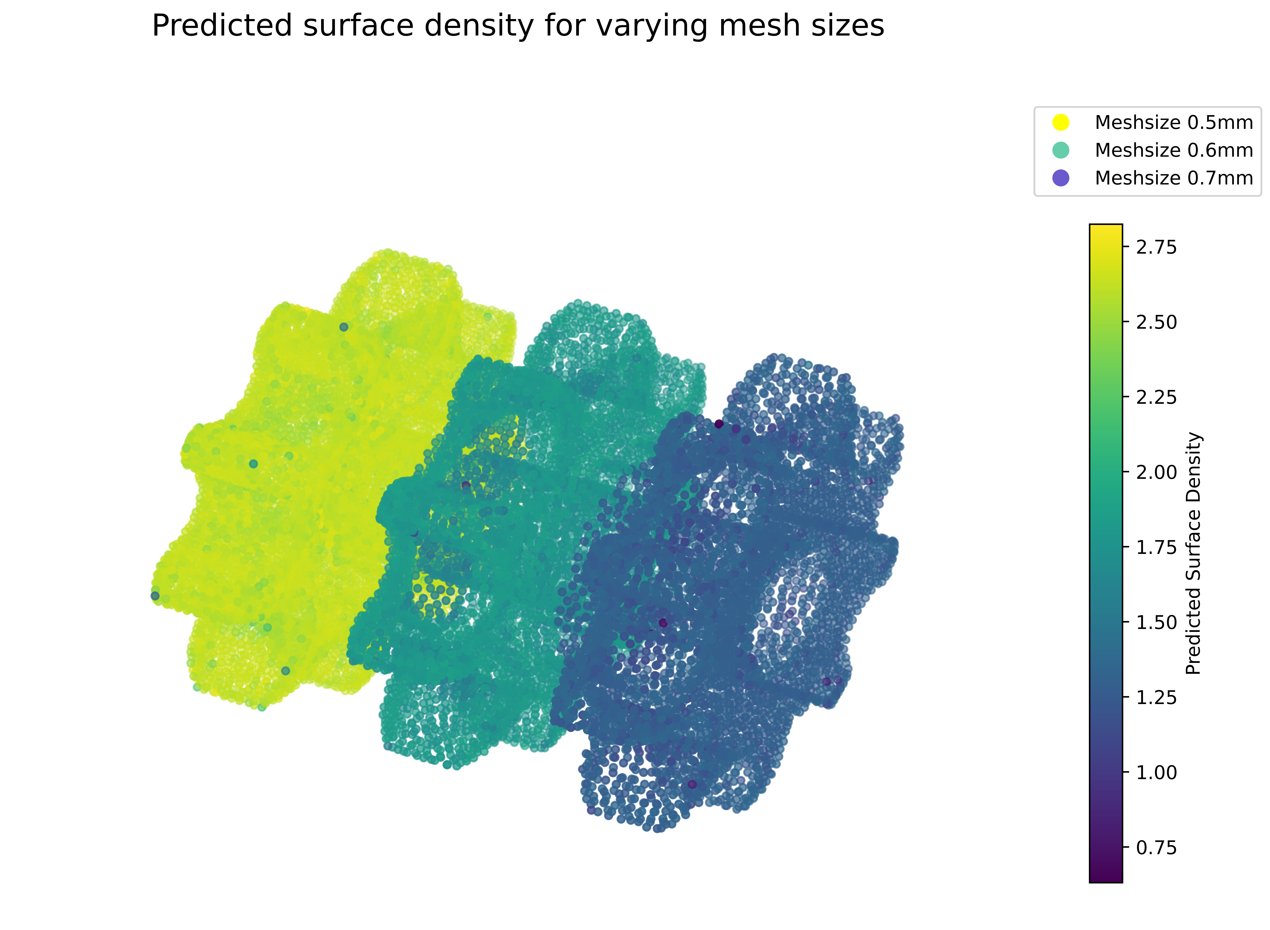
\includegraphics[width=0.5\textwidth]{figures/varying_meshsize_lowQ.png}
\caption{Surface density predictions for mesh sizes 0.5 mm, 0.6 mm, and 0.7 mm.}
\label{fig:diff_mesh_predict}
\end{figure}